\documentclass{article}
\usepackage{graphicx} % Required for inserting images
\usepackage{authblk}
\usepackage{cite}
\usepackage{natbib}
\usepackage{dcolumn}
\usepackage{pdfpages}
\usepackage{epigraph} % Required for inspirational quote
% packages required for kable()
\usepackage{booktabs}
\usepackage{longtable}
\usepackage{array}
\usepackage{multirow}
\usepackage{wrapfig}
\usepackage{float}
\usepackage{colortbl}
\usepackage{pdflscape}
\usepackage{tabu}
\usepackage{threeparttable}
\usepackage{threeparttablex}
\usepackage[normalem]{ulem}
\usepackage{makecell}
\usepackage{xcolor}
\renewcommand{\epigraphsize}{\small}
\setlength{\epigraphwidth}{0.51\textwidth}
\renewcommand{\textflush}{flushright}
\renewcommand{\sourceflush}{flushright}

% display code
\usepackage{listings}
\usepackage{color}

\definecolor{dkgreen}{rgb}{0,0.6,0}
\definecolor{gray}{rgb}{0.5,0.5,0.5}
\definecolor{mauve}{rgb}{0.58,0,0.82}
\lstset{frame=tb,
  language=Java,
  aboveskip=3mm,
  belowskip=3mm,
  showstringspaces=false,
  columns=flexible,
  basicstyle={\small\ttfamily},
  numbers=none,
  numberstyle=\tiny\color{gray},
  keywordstyle=\color{blue},
  commentstyle=\color{dkgreen},
  stringstyle=\color{mauve},
  breaklines=true,
  breakatwhitespace=true,
  tabsize=3
}


%\date{Draft -- please do not circulate.}

\title{(In)civility on Display: Social Media Discourse through the Ideological Lens}

\author[1]{David Broska}
%\author[2]{Byungkyu Lee}
%\author[3]{Barum Park}
%\author[4]{Daniel A. McFarland}
%\affil[1,4]{Stanford University}
%\affil[2]{New York University}
%\affil[2]{Cornell University}

\begin{document}

\maketitle

\begin{abstract}
Conversations are at the heart of democracies. Civil conversations – i.e., those based on mutual respect and critical engagement – help identify solutions to problems, avoid violent conflict, and foster a better understanding of each other. Existing literature does not sufficiently address how the broader public applies norms to conversations, and the social and psychological factors that shape the perceptions of conversations are not well understood. This project studies the determinants of perceived civility – and toxicity in particular – in the context of the 2016 US presidential election campaign, a time of rapidly changing conservational norms. Across 9,994 conversations in political Facebook groups, I study how 4,675 American survey respondents evaluate Facebook comments in terms of perceived toxicity. I find that, on average, liberals are more likely than conservatives to consider a comment as disrespectful, hateful, or otherwise conducive to making someone leave a conservation. However, this relationship varies across topics, with liberals perceiving comments that support abortion, immigration, and politicians of the Democratic party as less toxic. Conversely, conservatives perceive comments as more toxic when they are suggestive, endorse immigration, and portray the United States or white people negatively.
\end{abstract}
\clearpage

\epigraph{Civility costs nothing and buys everything.}{Mary Wortley Montagu 1756}
\epigraph{Civility is on the ballot.}{Barack Obama 2016}
%Respect for women is on the ballot. Tolerance is on the ballot. Justice is on the ballot. Equality is on the ballot. Democracy is on the ballot.

\section{Introduction}

Conversations are at the heart of democracies. Discussions in parliaments, the media, and everyday interactions inform political processes, help identify solutions to problems, avoid violent conflict, and foster a better understanding of each other. Some consider conversations based on reason rather than content and ignorance even a benchmark for achieving a democracy \citep{sanders_against_1997}. Attaining these desirable outcomes requires \textit{civility} from the interlocutors because it sets the stage for productive conversations. 
At a minimum,  civility means ``demonstrating mutual respect" \citep{mutz_inyourface_2016} or ``politeness" \citep{frimer_montagu_2018}. A maximalist definition of civility does not only require being respectful and polite but also critical engagement \citep{kant_enlightenment_1784}\footnote{Kant does not only argue that individuals should not only have the freedom but also the courage to make use of their own understanding -- i.e., to actively engage. For example, the clergyman is required to teach lessons aligned with the ``creed of the church he serves, for he was employed by it on that condition. But as a scholar he has complete freedom and is even called upon to communicate to the public all his carefully examined and well-intentioned thoughts about what is erroneous in that creed and his suggestions for a better arrangement of the religious and ecclesiastical body."} and requires individuals to give rationales in conversation \citep{habermas1985theory}. In other words, this expanded definition of civility demands contributions to conversations to be productive above and beyond avoiding offense.

While this distinction is grounded in theoretical traditions, it remains unclear how these perspectives align with the public's perception of desirable norms in conversations. Civility is a \textit{social praxis} embedded in what people know, who they are, what they do, and what they value. Extant literature does not sufficiently address how the broader public applies norms to conversations, and the social and psychological factors that shape the perceptions of conversations are not well understood. Most research focuses on politeness, coinciding with the shift of social media platforms to increase engagement with the side effect of amplifying the visibility of problematic behavior online (see Figure \ref{fig:n-gram}). Relatively little research sought to understand what constitutes constructive comments and how this benefits the overall conversation (cf. \citealp{mizil2016conversational}). We propose that politeness is only one dimension of civility, and perhaps only its minimal requirement. In this project, we consider constructiveness as an additional dimension of civility. \textit{What defines a polite and a constructive contribution to a discussion, respectively? How do these dimensions of civility shape whether a conversation is perceived as productive?}

This project studies civility in the context of the 2016 US presidential election campaign. Across 9,994 conversations held between 2015 and 2017 in political Facebook groups, we study how 4,675 American survey respondents evaluate comments given by discussants. The 2016 presidential campaign is an insightful case for the study of conversational norms because the discussions happened ``during a time of rapidly changing norms of political civility" \citep{munger_dont_2021}, and these exchanges were experienced ``first-hand" through broadcasting and online \citep{mutz_inyourface_2016}. Studying social media around this time offers a unique lens into the public sphere because an estimated 68\% of US adults were on a social network, up from 25\% in 2008 \citep{duggan_social_2016}. 



%Second, much research studying conservation online emphasized attitudinal differences without consideration of the form of the conversation. For example, political partisanship dispositions individuals to perceive the same stimulus differently \citep{vanbavel2018brain} and increases engagement with content about the political outgroup \citep{rathje2021outgroup}. Here, the idea the perception of a conversation is not the image created from a camera obscura that closely tracks how conversations unfold and the conversational dynamics within them. Rather, it is a camera obscur\textit{ed}, with the individual perception being subject to biases. 

%Remiss is conservation of the conversational form and how the 
%For this manuscript, we will focus on perceived toxicity, defined as a comment considered disrespectful, hateful, or that makes someone more likely to leave a discussion or give up sharing their perspective. 

\begin{figure}
    \centering
    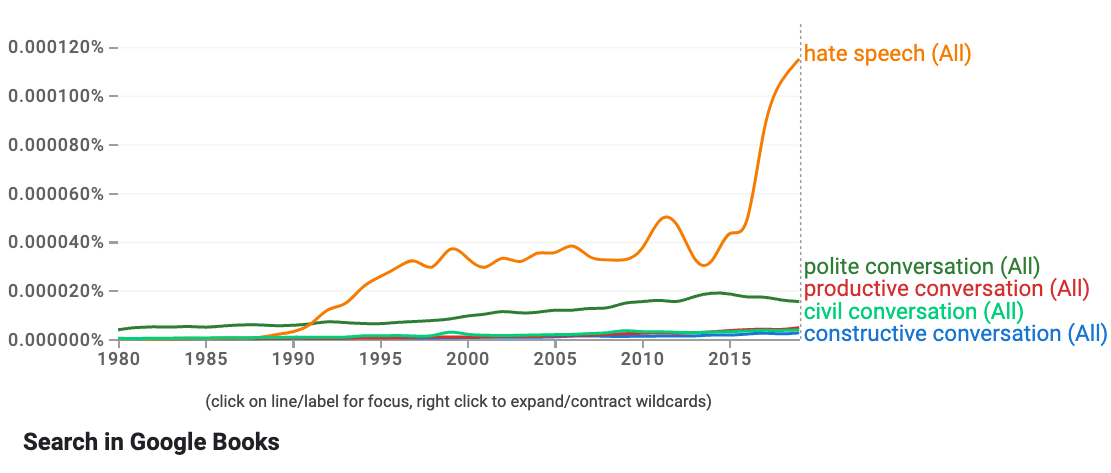
\includegraphics[width=1\linewidth]{figures/ngram.png}
    \caption{Google n-gram showing keywords related to civil conversations}
    \label{fig:n-gram}
\end{figure}

% https://books.google.com/ngrams/graph?content=constructive+conversation%2Cproductive+conversation%2Cpolite+conversation%2Chate+speech%2Ccivil+conversation&year_start=1985&year_end=2019&corpus=en-US-2019&smoothing=0


%While there was once hope that social media could advance democratic deliberation through open discourse, diverse perspectives, and broad participation, many observers note that social media discussions lack the crucial ingredient of civility. Concerns about declining civility are not new. From the printing press during the Reformation \citep{bejan_mere_2017} to the invention of cable news with its personalized news reporting \citep{mutz_inyourface_2016,berry2014outrage}, history is filled with examples of concerns about incivility of discourse. However, the 2016 US presidential election may have marked another critical turning point in recent history. 

\section{Hypotheses}

The main argument so far has been that politeness is only one dimension of civility but that a productive conversation depends on both politeness and constructive comments. I will conduct a mediation analysis to assess this claim. 
\begin{itemize}
    \item \textit{Total effect:} Perceived constructiveness of a comment is positively associated with productive conversations. 
    \item \textit{Indirect effect:} Politeness partially -- but not completely -- mediates the association between constructiveness and productiveness. 
    \item \textit{Direct effect:} The direct effect remains nonzero after including the mediator (politeness). 
\end{itemize}

Estimating this mediation model requires estimating the latent constructs of perceived politeness and constructiveness. I will discuss the steps taken in the Methods section below. 

\section{Data}

To study the determinants of perceived civility in conversations, we recruit 4,675 American adults via Prolific to fill out a survey asking them to evaluate Facebook conversations regarding perceived toxicity and other features. Respondents who did not pass an attention check were not allowed to take the survey. Excluding missing values\footnote{There is no evidence of differential attrition.}, the total sample size is 32,597 observations. Those who passed the attention check were randomly assigned to evaluate 7 conversations. Not every respondent evaluated each conversation; each one was evaluated 3.27 times on average. 

The 9,994 conversations are a stratified random sample of conversations from 1,058 public Facebook pages retrieved during the 2016 US presidential campaign via the official Facebook API v2.7. To ensure variation across the ideological spectrum on Facebook, we first obtained a list of the 500 most active political pages of the platform according to \citet{bakshy_exposure_2015}, as well as 37 pages identified as representative online and offline news sources by Pew Research Center’s American Trends Panel in 2014. These pages make up our media samples.

Table \ref{tab:summ-tab-ind} in the Supplementary Material provides summary statistics of the characteristics of survey respondents. Compared to demographic quotas from the American National Election Studies (ANES), this sample of 4,675 adults recruited via Prolific consists of more college-educated individuals (+10.7 percentage points) than those with a high school degree or less (-7.3pp). We over-sampled Democrats (+10.7pp) and under-sampled Republicans (-14.6pp). Finally, we over-sampled those aged 33 to 44 (+9.4pp), and under-sampled those aged 60 and older (-12.3pp). The sample is otherwise representative on these demographic dimensions. In a future analysis, we will consider whether results change if post-stratification techniques are applied, allowing us to make more credible inferences about the population of American adults.

\section{Methods}

We use structural equation modeling (SEM) to construct latent factors like politeness and constructiveness with a factor. The key advantage of this statistical framework is that it allows for the simultaneous estimation of multiple relationships and accounts for measurement errors, providing a more accurate and comprehensive understanding of the underlying constructs \citep{kline_principles_2016}. We therefore use SEM also to conduct a mediation analysis, implemented with the statistical software lavaan. This dual application of SEM enhances the robustness of the results by integrating measurement and estimate into a single framework.

I will conduct the proposed analysis in the following three steps. I will first conduct the factor analysis individually for each latent construct. Second, I will simultaneously estimate the latent factors of politeness and constructiveness. Finally, I will add the mediation analysis to the structural equation model. (ADD INFORMATION ABOUT MODEL FIT)

\section{Results}

\begin{table}[H]
\centering
\caption{\label{tab:sem-fit-measures}Fit measures for SEM models. All p-values for chi-squared test are smaller than 0.001}
\centering
\begin{tabular}[t]{lccccc}
\toprule
Model & chisq & df & rmsea & cfi & srmr\\
\midrule
Mediation & 5483.38 & 22 & 0.09 & 0.97 & 0.08\\
\cmidrule{1-6}
Constructive & 4457.61 & 16 & 0.09 & 0.97 & 0.08\\
\cmidrule{1-6}
Politeness & 589.37 & 2 & 0.09 & 0.99 & 0.06\\
\cmidrule{1-6}
Constructive & 4457.61 & 16 & 0.09 & 0.97 & 0.08\\
\bottomrule
\end{tabular}
\end{table}





\section{Conclusion and Discussion}


\newpage
\bibliographystyle{asr}
\bibliography{bib}

\clearpage
\section{Supplementary Material}

\begin{table}[htbp]
    \centering
    \begin{tabular}{|c|c|c|c|}
    \hline
    \textbf{Respondent Id} & \textbf{Post Id} & \textbf{Comment A Id} & \textbf{Comment B Id} \\
    \hline
    R1 & P2 & A2 & B2 \\
    R1 & P4 & A4 & B4 \\
    R1 & P23 & A23 & B23 \\
    R1 & P5 & A5 & B5 \\
    R1 & P56 & A56 & B56 \\
    R1 & P6 & A6 & B6 \\
    \midrule
    R2 & P4 & A4 & B4 \\
    R2 & P22 & A22 & B22 \\
    R2 & P6 & A6 & B6 \\
    R2 & P7 & A7 & B7 \\
    R2 & P9994 & A9994 & B9994 \\
    R2 & P11 & A11 & B11 \\
    R2 & P55 & A55 & B55 \\
    \midrule
    \dots & \dots & \dots & \dots \\
    \hline
    \end{tabular}
    \caption{Sample table to illustrate the nested data structure}
    \label{sample-table}
\end{table}

\clearpage

% Dependent variable plot 

\begin{figure}[h]
    \centering
    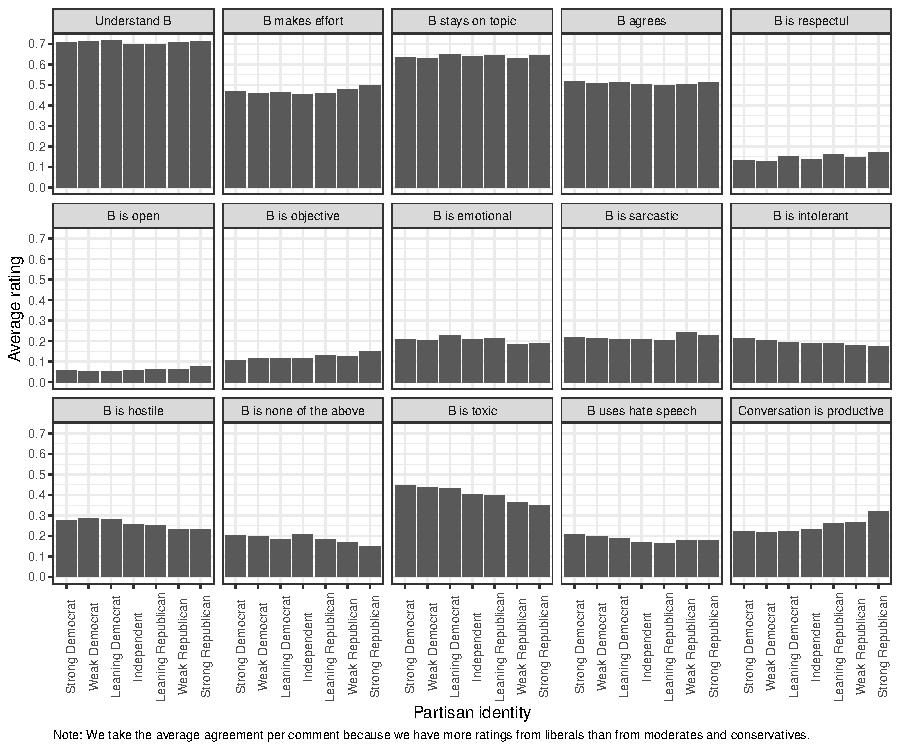
\includegraphics[width=1\linewidth]{figures/2_AvgAgreement_Partisanship.pdf}
    \caption{Variables measuring dimensions of civility by partisanship}
    \label{fig:civility-partisanship}
    \vspace{0.25cm}
    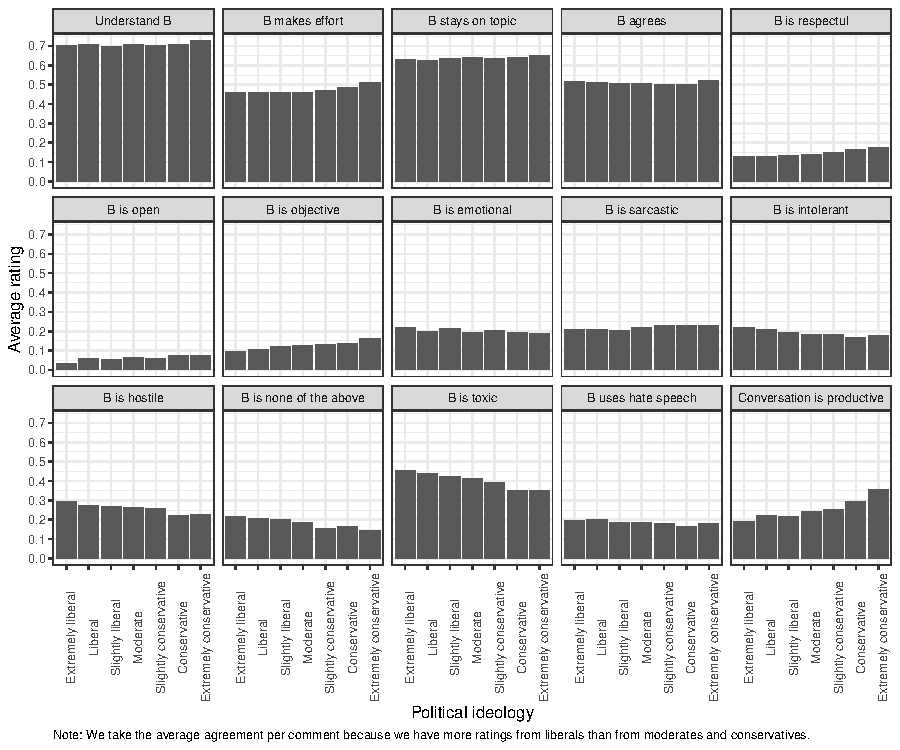
\includegraphics[width=1\linewidth]{figures/2_AvgAgreement_Ideo.pdf}
    \caption{Variables measuring dimensions of civility by political ideology}
    \label{fig:civility-ideology}
\end{figure}
\clearpage
%%%%%%%%%%%%%%%%%%%%%%%%%%%%%%%%%%%%%%%%%%
% Summary statistics % 
\renewcommand{\arraystretch}{0.9}
\begin{table}[!h]
\centering
\caption{\label{tab:summ-tab-ind}Summary statistics on characteristics of survey respondents}
\centering
\begin{tabular}[t]{llrrrrrr}
\toprule
Type & Variable & Min & Q25 & Mean & Median & Q75 & Max\\
\midrule
Dependent Variable & BToxicNum01 & -0.42 & -0.42 & 0.00 & -0.08 & 0.25 & 0.58\\
\cmidrule{1-8}
 & PolIdComp & 1.00 & 1.50 & 3.18 & 3.00 & 4.50 & 7.00\\
\cmidrule{2-8}
 & PolIdComp2Sd & -0.61 & -0.47 & 0.00 & -0.05 & 0.37 & 1.07\\
\cmidrule{2-8}
 & Man & 0.00 & 0.00 & 0.49 & 0.00 & 1.00 & 1.00\\
\cmidrule{2-8}
 & Woman & 0.00 & 0.00 & 0.48 & 0.00 & 1.00 & 1.00\\
\cmidrule{2-8}
 & OtherGender & 0.00 & 0.00 & 0.02 & 0.00 & 0.00 & 1.00\\
\cmidrule{2-8}
 & EducationNum & 1.00 & 3.00 & 3.05 & 3.00 & 3.00 & 5.00\\
\cmidrule{2-8}
 & Income2Sd & -0.58 & -0.30 & 0.00 & -0.13 & 0.38 & 1.79\\
\cmidrule{2-8}
 & Asian & 0.00 & 0.00 & 0.07 & 0.00 & 0.00 & 1.00\\
\cmidrule{2-8}
 & Black & 0.00 & 0.00 & 0.15 & 0.00 & 0.00 & 1.00\\
\cmidrule{2-8}
 & Hispanic & 0.00 & 0.00 & 0.08 & 0.00 & 0.00 & 1.00\\
\cmidrule{2-8}
 & White & 0.00 & 1.00 & 0.76 & 1.00 & 1.00 & 1.00\\
\cmidrule{2-8}
 & OtherRace & 0.00 & 0.00 & 0.03 & 0.00 & 0.00 & 1.00\\
\cmidrule{2-8}
 & Married & 0.00 & 0.00 & 0.39 & 0.00 & 1.00 & 1.00\\
\cmidrule{2-8}
 & Separated & 0.00 & 0.00 & 0.01 & 0.00 & 0.00 & 1.00\\
\cmidrule{2-8}
 & Widowed & 0.00 & 0.00 & 0.02 & 0.00 & 0.00 & 1.00\\
\cmidrule{2-8}
 & MaritalNoAnswer & 0.00 & 0.00 & 0.02 & 0.00 & 0.00 & 1.00\\
\cmidrule{2-8}
 & Divorced & 0.00 & 0.00 & 0.10 & 0.00 & 0.00 & 1.00\\
\cmidrule{2-8}
 & NeverMarried & 0.00 & 0.00 & 0.46 & 0.00 & 1.00 & 1.00\\
\cmidrule{2-8}
 & EvangelicalProtestant & 0.00 & 0.00 & 0.11 & 0.00 & 0.00 & 1.00\\
\cmidrule{2-8}
 & MainlineProtestant & 0.00 & 0.00 & 0.11 & 0.00 & 0.00 & 1.00\\
\cmidrule{2-8}
 & Mormon & 0.00 & 0.00 & 0.01 & 0.00 & 0.00 & 1.00\\
\cmidrule{2-8}
 & Catholic & 0.00 & 0.00 & 0.16 & 0.00 & 0.00 & 1.00\\
\cmidrule{2-8}
 & Jewish & 0.00 & 0.00 & 0.02 & 0.00 & 0.00 & 1.00\\
\cmidrule{2-8}
 & Muslim & 0.00 & 0.00 & 0.01 & 0.00 & 0.00 & 1.00\\
\cmidrule{2-8}
 & NotReligious & 0.00 & 0.00 & 0.00 & 0.00 & 0.00 & 0.00\\
\cmidrule{2-8}
 & ReligionNoAnswer & 0.00 & 0.00 & 0.00 & 0.00 & 0.00 & 0.00\\
\cmidrule{2-8}
\multirow{-27}{*}{\raggedright\arraybackslash Demographics} & OtherReligion & 0.00 & 0.00 & 0.09 & 0.00 & 0.00 & 1.00\\
\bottomrule
\end{tabular}
\end{table}


\clearpage
% End summary statistics 
%%%%%%%%%%%%%%%%%%%%%%%%%%%%%%%%%%%%%%%%%%%%




\end{document}

